%! Author = Robert Kulesa, Daniel Liu, Michael Li
%! Date = 11/4/2021

% Preamble
\documentclass[11pt]{article}

% Packages
\usepackage{amsmath}
\usepackage{graphicx}

% Document
\begin{document}
    \begin{titlepage}
        \begin{center}
            \vspace{1cm}

            \Huge
            \textbf{Search Problems in AI}

            \vspace{0.5cm}
            \LARGE
            Assignment 2

            \vspace{1cm}

            \textbf{Michael Li - 192008938}

            \textbf{Daniel Liu - 184007283}

            \textbf{Robert Kulesa - 185009892}


            \vfill


            \vspace{0.8cm}

            \Large
            CS440 Fall 2021\\
            Professor Boularias\\
            Rutgers University - New Brunswick\\
            November 12, 2021

        \end{center}
    \end{titlepage}

    \begin{center}
        \Large
        \textbf{Problem 1}
    \end{center}
    \normalsize
    The sequence of nodes expanded by A* search, given the tree,
    and straight line distance heuristics, is in the following order:
    \begin{enumerate}
        \item[0.] $\left(city, f(city), g(city), h(city)\right)$
        \item $\left(\text{Lugoj}, 244, 0, 244\right)$
        \item $\left(\text{Mehadia}, 311, 70, 241\right)$
        \item $\left(\text{Lugoj}, 384, 140, 244\right)$
        \item $\left(\text{Drobeta}, 387, 145, 242\right)$
        \item $\left(\text{Craiova}, 425, 265, 160\right)$
        \item $\left(\text{Timisoara}, 440, 111, 329\right)$
        \item $\left(\text{Mehadia}, 451, 210, 241\right)$
        \item $\left(\text{Mehadia}, 461, 220, 241\right)$
        \item $\left(\text{Lugoj}, 466, 222, 244\right)$
        \item $\left(\text{Pitesti}, 503, 403, 100\right)$
        \item $\left(\text{Bucharest}, 504, 504, 0\right)$
    \end{enumerate}

    \begin{center}
        \Large
        \textbf{Problem 2}
    \end{center}
    \normalsize
    \begin{enumerate}
        \item[(a)] %insert explanation here
          BFS: $1 \rightarrow 2 \rightarrow 3\rightarrow 4 \rightarrow 5 \rightarrow 6 \rightarrow 7 \rightarrow 8 \rightarrow9\rightarrow10\rightarrow11$\\
          DLS: $1\rightarrow2\rightarrow4\rightarrow8\rightarrow9\rightarrow5\rightarrow10\rightarrow11$\\
          IDS: \\
          $1$\\
          $1\rightarrow2\rightarrow3$\\
          $1\rightarrow2\rightarrow4\rightarrow5\rightarrow3\rightarrow6\rightarrow7$\\
          $1\rightarrow2\rightarrow4\rightarrow8\rightarrow9\rightarrow5\rightarrow10\rightarrow11$
        
        \item[(b)] %insert explanation here\\
        Bidirectional search would be effective in solving this problem.
        Bidirectionally finding a path between state 1 and state 11 reduces
        the number of nodes that needs to be explored.
        
        Forward   1\\
        Backward  11\\
        Forward   2\\
        Backward  5
        
        The branching factor is 2 in the forward direction and 1 in the reverse direction.
        
    \end{enumerate}

    \begin{center}
        \Large
        \textbf{Problem 3}
    \end{center}
    \normalsize
    \begin{enumerate}
        \item[(a)] True
        \item[(b)] True
        \item[(c)] True
        \item[(d)] False
        \item[(e)] False
        \item[(f)] True
        \item[(g)] True
        \item[(h)] False
        \item[(i)] True
    \end{enumerate}

    \begin{center}
        \Large
        \textbf{Problem 4}
    \end{center}
    \normalsize
    \begin{enumerate}
        \item[Advantage:]
        While the BFS algorithm has a space complexity of $\mathcal{O}(b^d)$, where $b$ is the tree branching factor
        and $d$ is the depth of the tree, the iterative deepening search algorithm (IDDFS) has a space complexity of $\mathcal{O}(bd)$.
        In short, IDDFS saves on space while still being complete.
        \item[Disadvantage:] IDDFS is slightly slower than BFS, since while nodes at the bottom of the search
        tree are only expanded once, the number of expansions for each node increments at each higher level in the tree.
    \end{enumerate}

    \begin{center}
        \Large
        \textbf{Problem 5}
    \end{center}
    \normalsize
    %insert explanation here
    a)\\
    A heuristic is considered consistent iff:\\
        $h(n) \leq c(n,n+1) + h(n+1)$\\
        where h() is the heuristic and n is the goal state\\
        Proving by induction with the $n-1$ node in the shortest path to $n$ (base step):\\
        $h(n-1) \leq c(n-1,n) + h(n)$\\
        since n is the goal state, $h(n)=h^*(n)$, where $h^*(n)$ is the true minimal cost to the goal state\\
        $h(n) \leq c(n-1,n) + h^*(n)$\\
        given $c(n-1) + h^*(n) = h^*(n-1)$\\
        $h(n-1) \leq h^*(n-1)$\\
        which is the definition of admissibility\\\\
        Inductive Step with $n-2$:\\
        $h(n-2) \leq c(n-2,n-1) + h(n-1)$\\
        drawing from the base case:\\
        $h(n-2) \leq c(n-2,n-1) + h(n-1) \leq c(n-2,n-1) + h^*(n-1)$\\
        $h(n-2)\leq c(n-2,n-1) + h^*(n-1)$\\
        $h(n-2) \leq h^*(n-2)$\\
        By inductive reasoning, consistency implies admissibility\\\\
    b)\\
    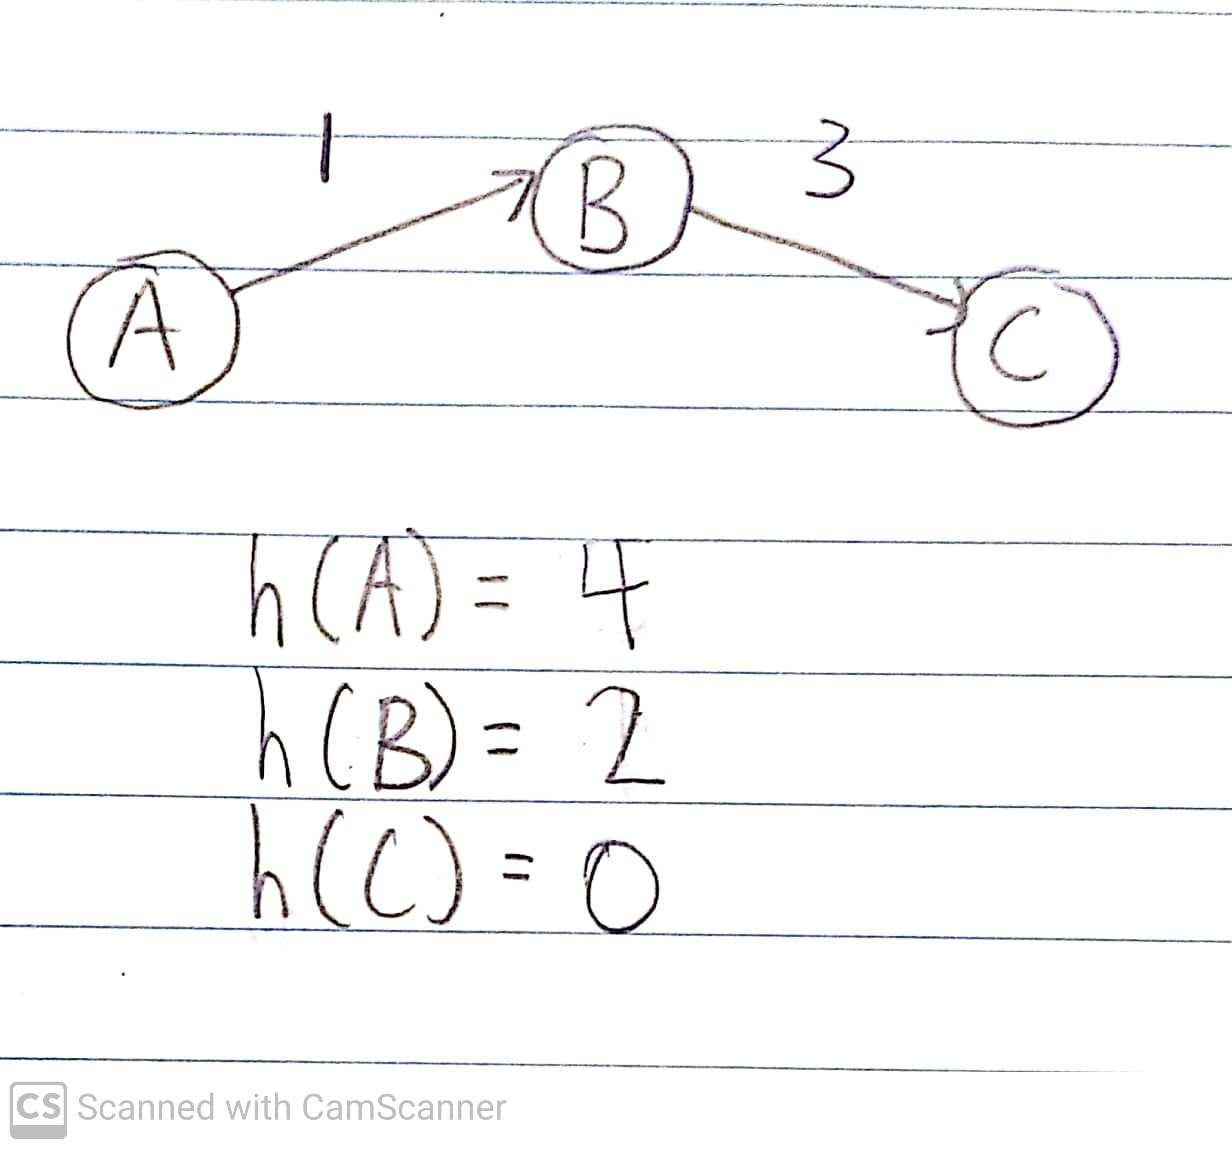
\includegraphics[width=0.9\textwidth]{images/prob_5_heuristic}
    
    \begin{center}
        \Large
        \textbf{Problem 6}
    \end{center}
    \normalsize
    In solving Constraint Satisfaction Problems, we choose the most constrained variable (MCV)
    in order to reduce the size of the next sub-problem.
    In other words, choosing the MCV maximally reduces the size of the next branch among
    any of the other variables. \\
    When assigning a value for this variable, we want to leave the remaining variables as unconstrained
    as possible in order to not accidentally eliminate any valid solutions.
    Thus, we want to assign the MCV the least constraining value (LCV).

    \begin{center}
        \Large
        \textbf{Problem 7}
    \end{center}
    \normalsize
    \begin{enumerate}
        \item[(a)]
            \begin{minipage}[!htb]{\linewidth}
                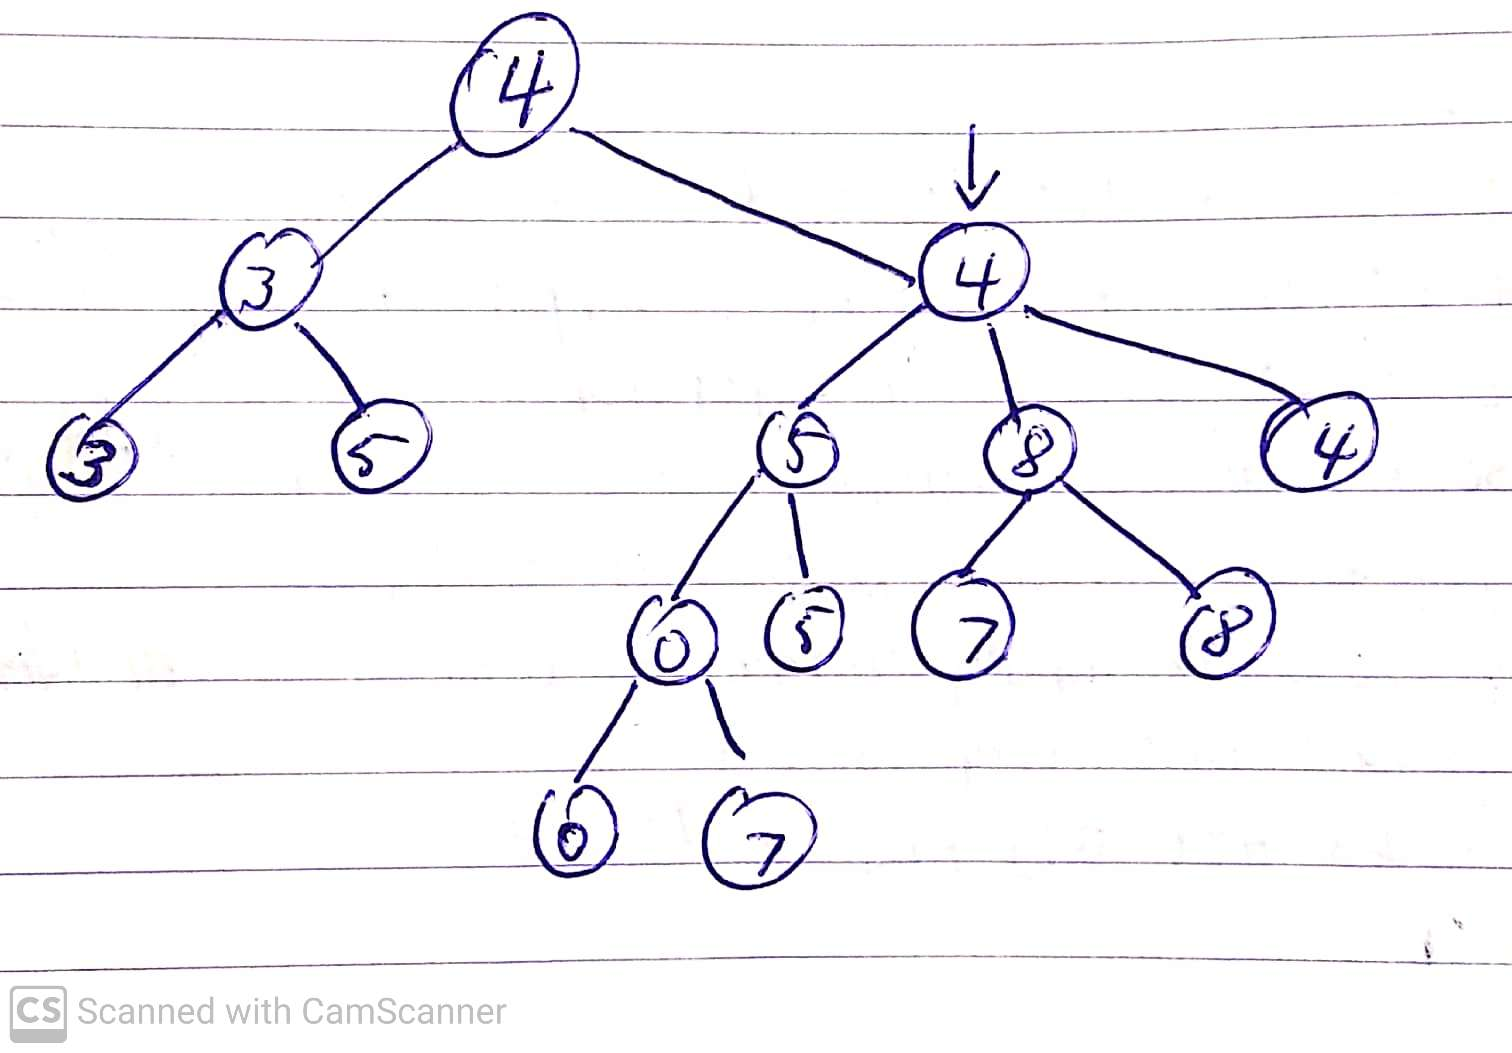
\includegraphics[width=\linewidth]{images/minmax_tree} \\
                The optimal choice for the max player would be the right node.
            \end{minipage}

        \item[(b)] %insert explanation here
            \begin{minipage}[!htb]{\linewidth}
                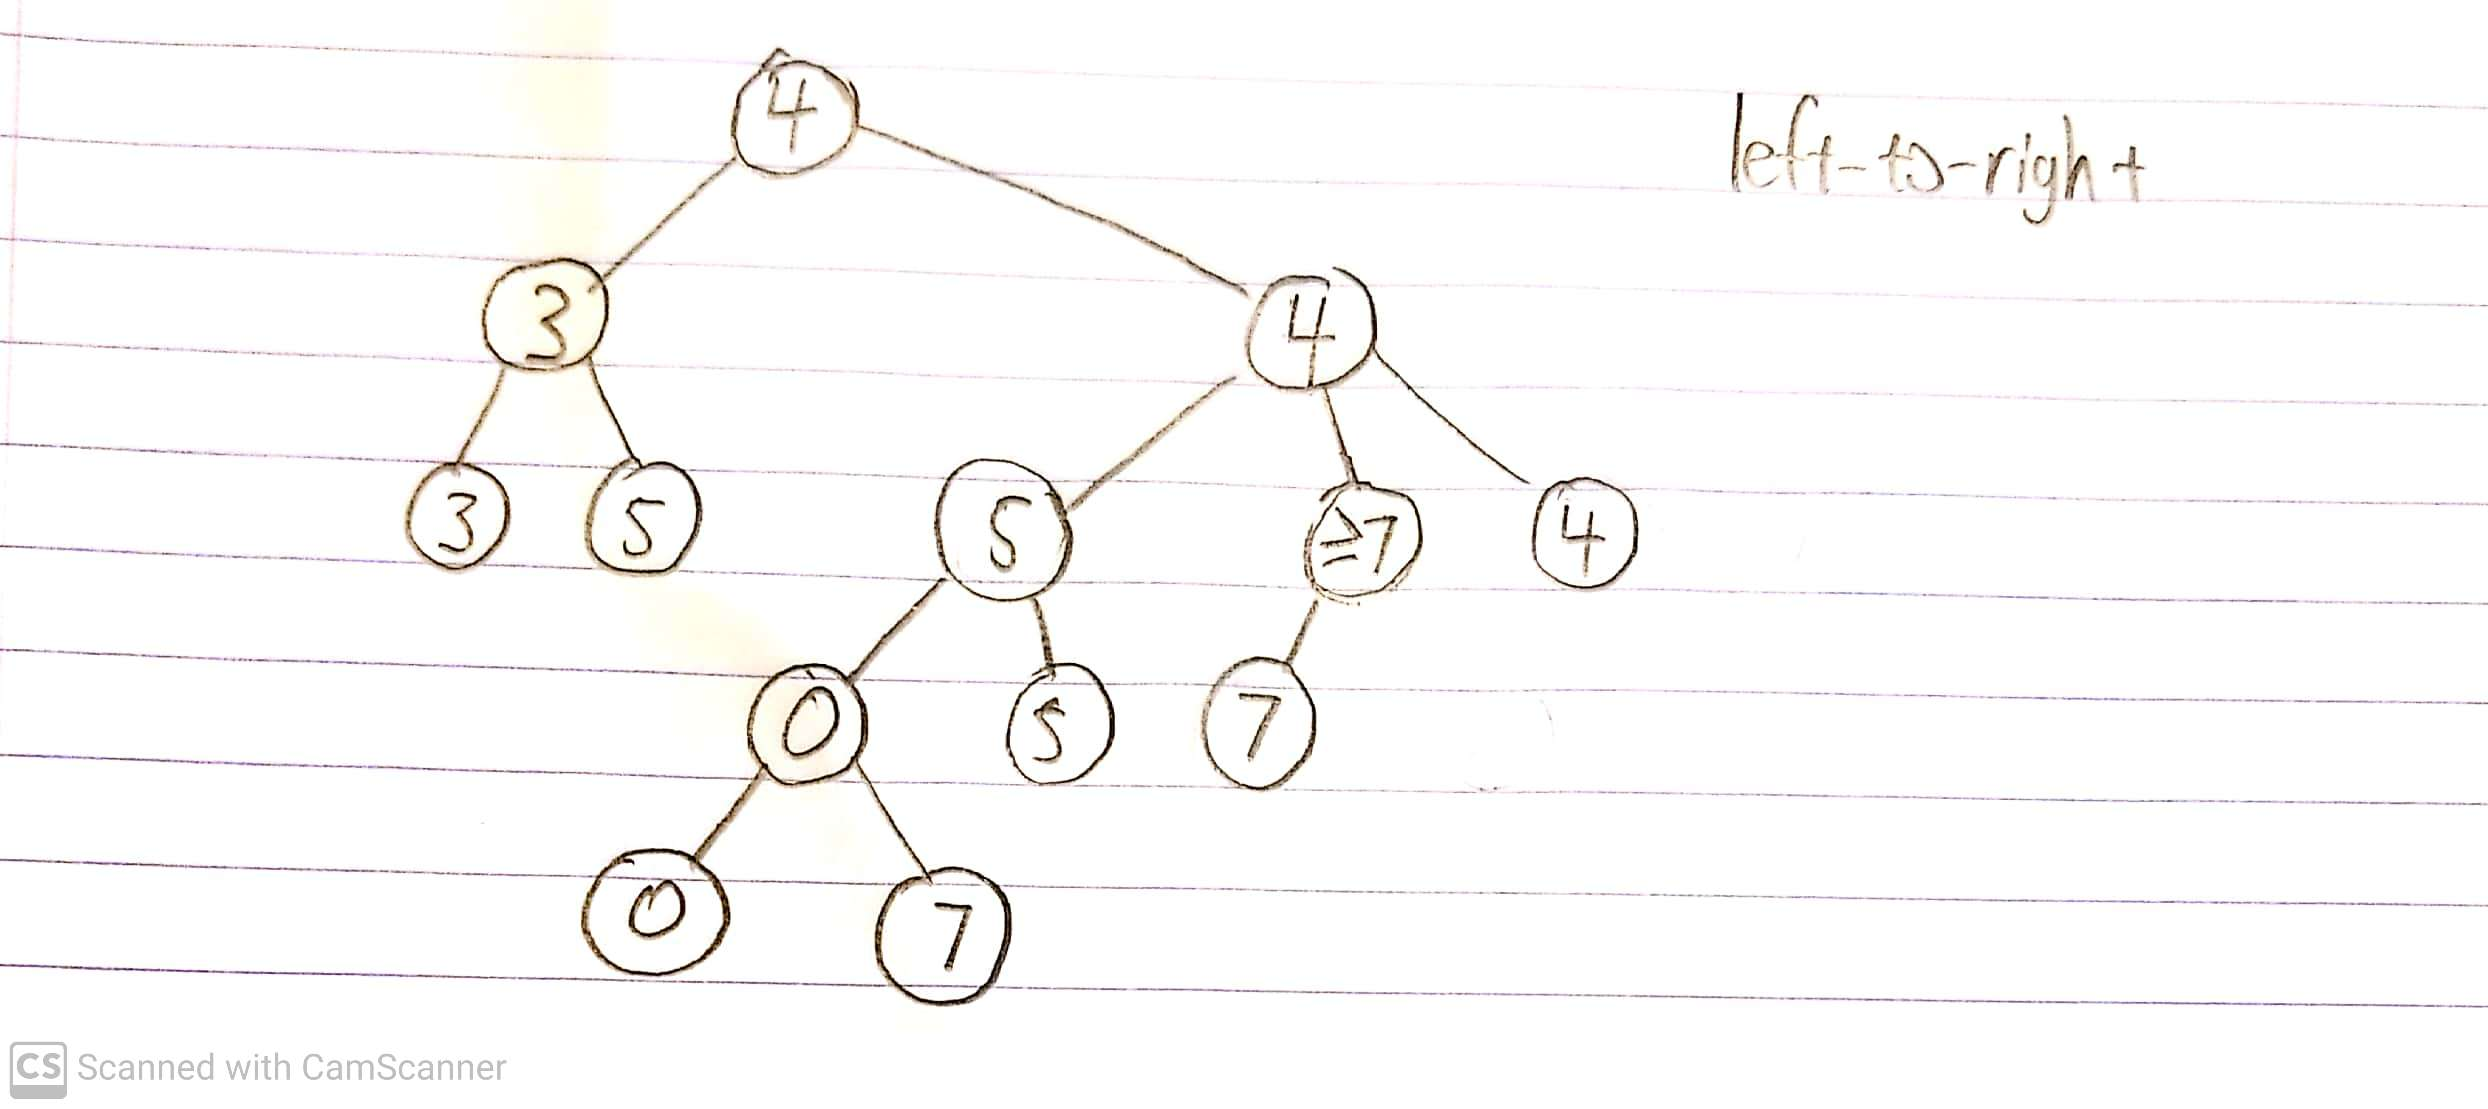
\includegraphics[width=\linewidth]{images/l2r_minmax_tree} \\
            \end{minipage}

        \item[(c)] %insert explanation here
            \begin{minipage}[!htb]{\linewidth}
                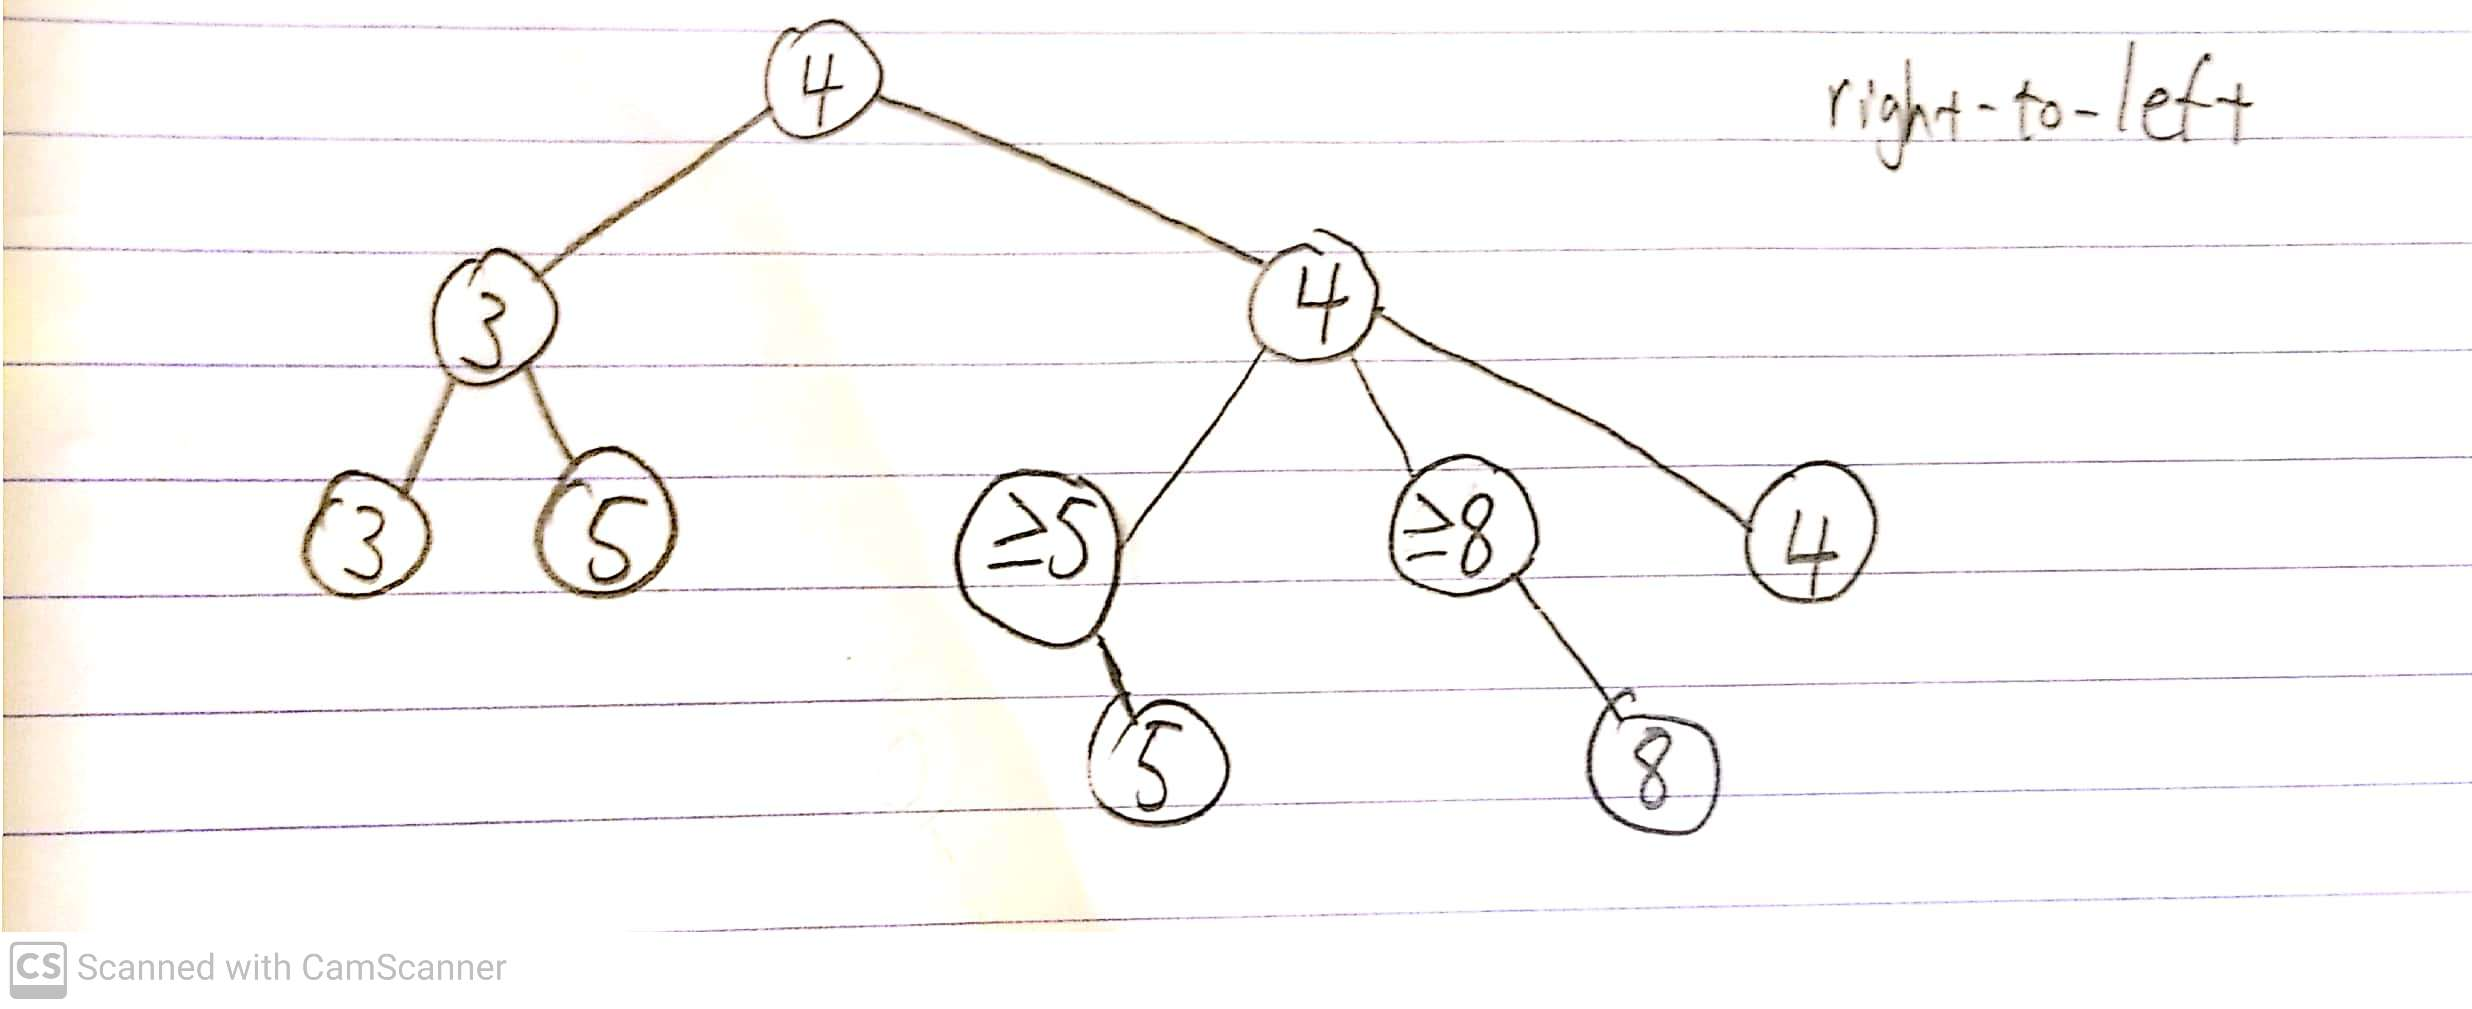
\includegraphics[width=\linewidth]{images/r2l_minmax_tree} \\
                Alpha-beta pruning is a heuristic that depends heavily on where elements are positioned, as it only operates on the best values found so far when exploring the tree. If the algorithm happens to find the 'best' node first then it can 'prune' more nodes from the tree. This is the case in right-to-left pruning, which, due to how the elements were positioned, was able to find the 'best' value more quickly and prune more nodes.
            \end{minipage}
    \end{enumerate}

    \begin{center}
        \Large
        \textbf{Problem 8}
    \end{center}
    \normalsize
    \begin{enumerate}
        \item[(a)]
            \begin{enumerate}
                \item[i.] Given both heuristics $h_1$ and $h_2$ are admissible,
                \[h(n) = min\{h_1(n), h_2(n)\}\] is an admissible heuristic.
                Since both heuristics never overestimate the true cost of getting to the target state, then choosing the minimum
                of these two heuristic values for each state is an admissible heuristic, as none of the
                new values will overestimate the true cost of getting to the target state.
                \item[ii.] Given both heuristics $h_1$ and $h_2$ are consistent: \\
                Since $h_1(n) \leq c(n, n') + h_1(n')$ and $h_2(n) \leq c(n, n') + h_2(n')$,
                \begin{gather*}
                    h(n) \leq min\{c(n, n') + h_1(n'), c(n, n') + h_2(n')\}\\
                    h(n) \leq min\{h_1(n'), h_2(n')\} + c(n, n')
                \end{gather*}
                Substituting $h(n')$ for $min\{h_1(n'), h_2(n')\}$,
                \[h(n) \leq h(n') + c(n, n')\]
                Thus, $h(n) = min\{h_1(n), h_2(n)\}$ is a consistent heuristic.
            \end{enumerate}

        \item[(b)]
            \begin{enumerate}
                \item[i.] Given both heuristics $h_1$ and $h_2$ are admissible,
                \[h(n) = wh_1(n)+(1-w)h_2(n)\] is an admissible heuristic.
                Since both heuristics never overestimate the true cost of getting to the target state, then choosing
                a value between these two heuristic values for each state is an admissible heuristic, as none of the
                new values will overestimate the true cost of getting to the target state.
                \item[ii.] Given both heuristics $h_1$ and $h_2$ are consistent: \\
                Since $h_1(n) \leq c(n, n') + h_1(n')$ and $h_2(n) \leq c(n, n') + h_2(n')$,
                \begin{gather*}
                    h(n) \leq w\left(c(n, n') + h_1(n')\right)+(1-w)\left(c(n, n') + h_2(n')\right)\\
                    h(n) \leq wh_1(n')+(1-w)h_2(n') + wc(n, n') + (1-w)c(n, n')\\
                    h(n) \leq wh_1(n')+(1-w)h_2(n') + c(n, n')
                \end{gather*}
                Substituting $h(n')$ for $wh_1(n)+(1-w)h_2(n)$,
                \[h(n) \leq h(n') + c(n, n')\]
                Thus, $h(n) = wh_1(n)+(1-w)h_2(n)$ is a consistent heuristic.
            \end{enumerate}

        \item[(c)]
            \begin{enumerate}
                \item[i.] Given both heuristics $h_1$ and $h_2$ are admissible,
                \[h(n) = max\{h_1(n), h_2(n)\}\] is an admissible heuristic.
                Since both heuristics never overestimate the true cost of getting to the target state, then choosing the maximum
                of these two heuristic values for each state is an admissible heuristic, as none of the
                new values will overestimate the true cost of getting to the target state.
                \item[ii.] Given both heuristics $h_1$ and $h_2$ are consistent: \\
                Since $h_1(n) \leq c(n, n') + h_1(n')$ and $h_2(n) \leq c(n, n') + h_2(n')$,
                \begin{gather*}
                    h(n) \leq max\{c(n, n') + h_1(n'), c(n, n') + h_2(n')\}\\
                    h(n) \leq max\{h_1(n'), h_2(n')\} + c(n, n')
                \end{gather*}
                Substituting $h(n')$ for $max\{h_1(n'), h_2(n')\}$,
                \[h(n) \leq h(n') + c(n, n')\]
                Thus, $h(n) = max\{h_1(n), h_2(n)\}$ is a consistent heuristic.
            \end{enumerate}
        \item[(d)] Heuristic C, $h(n) = max\{h_1(n), h_2(n)\}$, should be chosen.
        For consistent heuristics, higher cost estimation values (without going over) are better,
        as less states will be explored before reaching the goal state.
        Thus, a heuristic that chooses the maximum among two consistent heuristics for each state is preferred
        over the other options.
    \end{enumerate}

    \begin{center}
        \Large
        \textbf{Problem 9}
    \end{center}
    \normalsize
    \begin{enumerate}
        \item[(a)] 
        In problems that possess no local maxima in their cost function, hill climbing would work better. Hill climbing typically gets stuck within             local maxima. This is because in hill climbing, downward moves are prohibited, whereas in simulated annealing, downward moves are allowed               and thus, it is able to escape the local maxima.
        
        \item[(b)] %insert explanation here
        In problems where the cost function does not have any defined structure neighboring the global maximum is when randomly guessing the state                  will work as well as simulated annealing. This is because since there is no real structure, it is hard to determine a pattern and one                   would not know how to most efficiently reach the solution.
        \item[(c)] %insert explanation here
        In problems where the cost function possesses some local maxima along with having a defined overall global structure, simulated annealing               would be useful. 
        \item[(d)] %insert explanation here
        Instead of returning the current state at the end of the annealing schedule, we could create a maximum variable that will store the highest             value (measure of goodness) throughout the process. Should simulated annealing stop at a lower value, we will still be able to return the               maximum value, which will be the global maximum. 

        \item[(e)] %insert explanation here
        Since we have enough memory that we could hold two million states, instead of just storing the current state and the next proposed state, we            could instead store every state that we visit and mark them. We update the states should we find a higher value than the maximum so far. Once           the annealing schedule ends, should we end up with a current end value less than the maximum, we can return the maximum instead by looking              through our states that we have stored. 

        \item[(f)] %insert explanation here
        In simulated annealing, being trapped at a local maxima can be can avoided since it utilizes randomness that can either increase the objective          function or decrease it, allowing it to escape out of the maxima. The probability of decreases not as likely as increases, and gets less                likely as time goes on. We can adapt this randomness to gradient ascent to avoid local maxima by choosing the gradient randomly. Similar to               simulated annealing, should the gradient get stuck in a local maxima, the randomness will allow it to escape when the gradient is                         decreased at random.
    \end{enumerate}


\end{document}
